\documentclass[12pt]{beamer}
\usetheme{Boadilla}
\usepackage{graphicx}
\usepackage{algorithm2e}
\graphicspath{{images/}}
\title{CMPT 155: Computer Applications for Life Sciences}
\subtitle{Lecture 8:  Charts}
\author{Ivan E. Perez}
\date{February 11, 2022}
\usepackage{booktabs} % Allows the use of \toprule, 
\usepackage{appendix}
\usepackage{enumerate,multicol}
\usepackage{amsmath, amssymb, amsthm}
\usepackage{tikz}
\usepackage{amsxtra}
\begin{document}
	
	\begin{frame}
		\titlepage
	\end{frame}
	
	\begin{frame}
		\frametitle{Presentation Outline}
		\tableofcontents
	\end{frame}
	\section{Creating Charts}
	\begin{frame}
		\frametitle{Creating Charts}
		\begin{itemize}
			\item Download \textit{SimpleChart.xlsx} from moodle
			\item To create a charge select the range of cells including column and row headers (A1:B7)
			\item On the ribbon go to View $\rightarrow$ Charts, and select the appropriate chart! 
			\begin{itemize}
				\item whats the most appropriate chart for this dataset?
			\end{itemize}
			\begin{figure}[htb]
			\begin{minipage}[t]{0.5\linewidth}\centering
				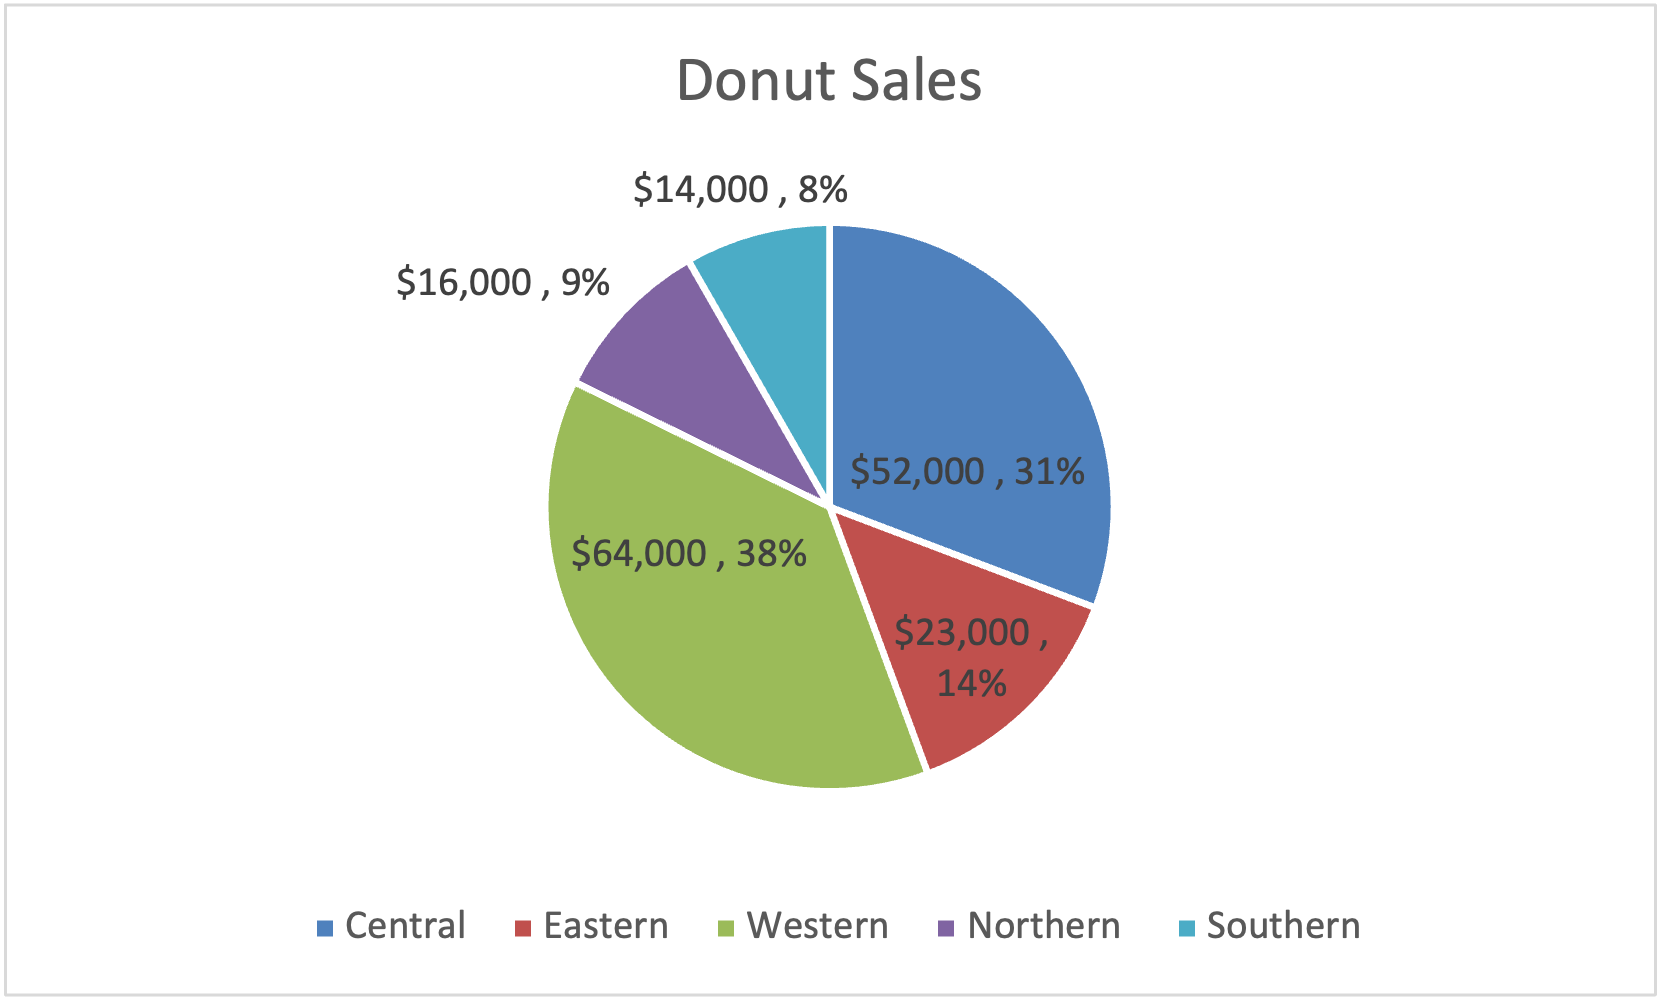
\includegraphics[width=0.9\linewidth]{SimpleChartPie.png}
				\medskip
				\centerline{(a)}
			\end{minipage}\hfill
			\begin{minipage}[t]{0.5\linewidth}\centering
				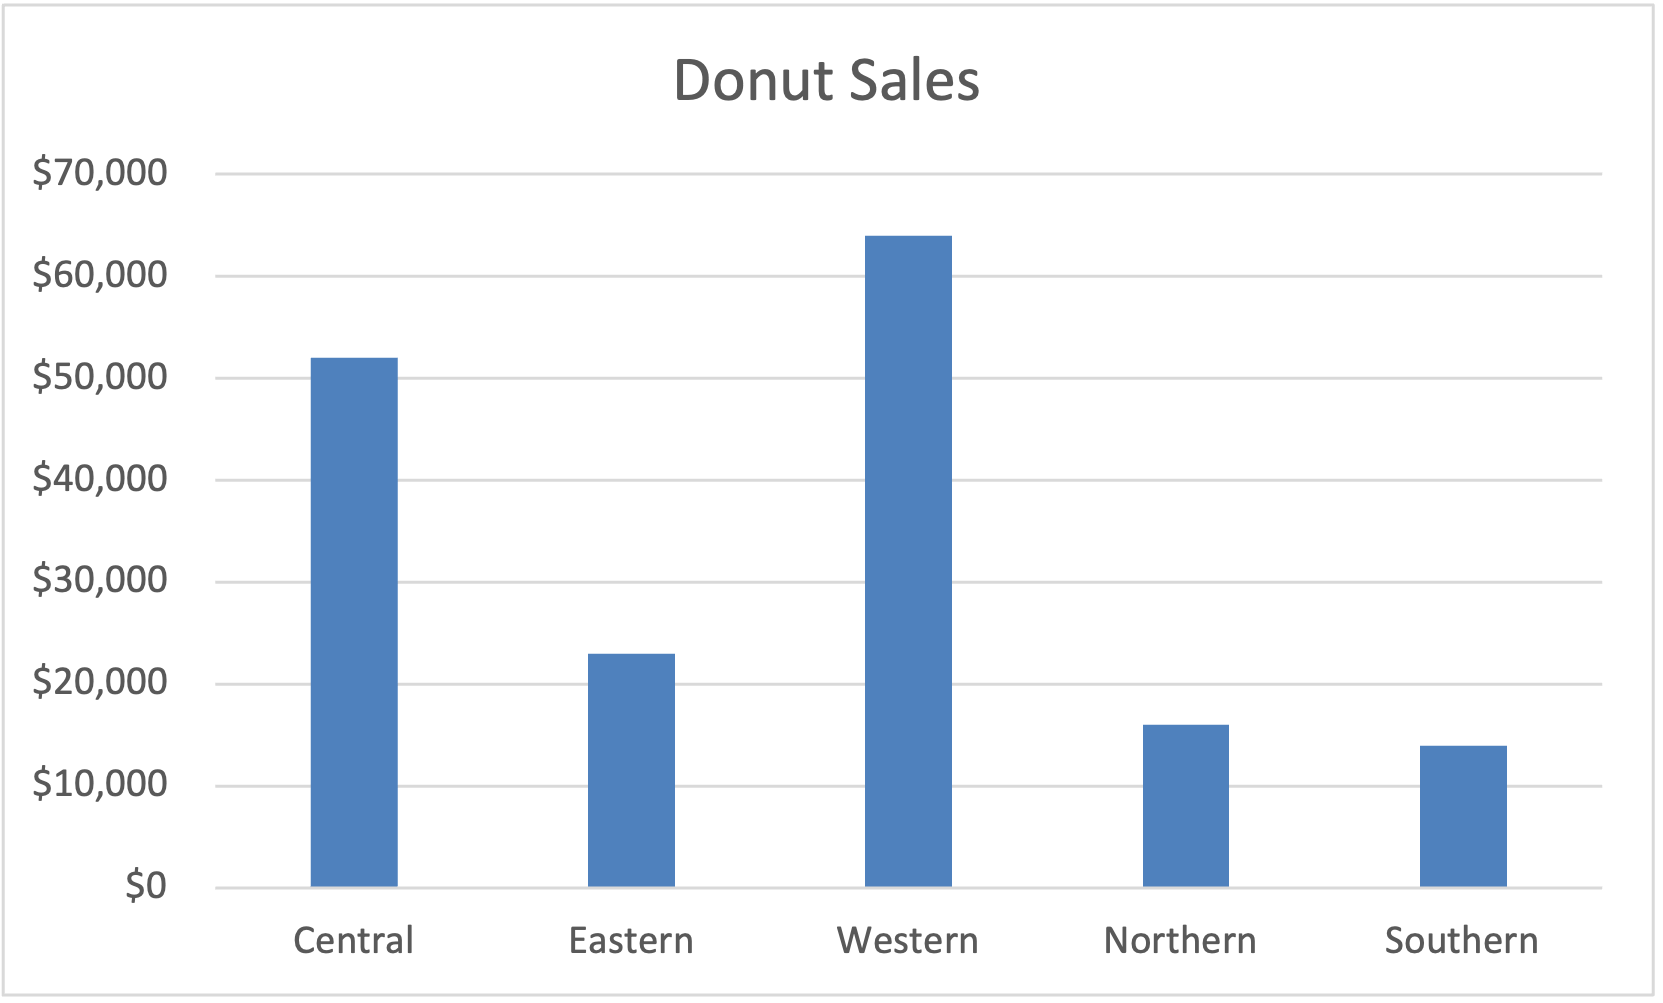
\includegraphics[width=0.9\linewidth]{SimpleChartBar.png}
				\medskip
				\centerline{(b)}
			\end{minipage}
			\caption{Pie and Bar chart representations of Donut Sales}
		\end{figure}
		\end{itemize}
	 
	\end{frame}

	\begin{frame}
		\frametitle{Changing Chart Types}
		\begin{itemize}
			\item You can change the chart type, by
			\begin{enumerate}
				\item right (Ctrl) clicking the chart 
				\item selecting ``Change Chart Type"
				\item clicking on appropriate chart type for the data selection
			\end{enumerate}
		\item What kinds of charts are appropriate for \textit{comparing data?}
		\end{itemize}
	\end{frame}

	\begin{frame}
		\frametitle{Chart Design Ribbon}
	The Chart Design tab in the Top Ribbon can be used to add and change chart elements.  
	\begin{itemize}
		\item Add Chart Element
		\begin{itemize}
			\item add individual elements (e.g., titles, legends, etc.)
		\end{itemize}
		\item Quick Layout
		\begin{itemize}
			\item modify current chart to have some preset chart elements
		\end{itemize}
		\item Change Colors
			\begin{itemize}
				\item Change the color palet of the chart 
			\end{itemize}
	\end{itemize}
\end{frame}
	\begin{frame}
		\frametitle{Chart Design Ribbon (continued)}
		\begin{itemize}
				\item Switch Row/Column
			\begin{itemize}
				\item Switches whether Excel will define a series using Rows or Columns.
				\item Used to look at different groupings of data.
			\end{itemize}
			\item Select data
			\begin{itemize}
				\item Specifies the exact cells referenced for a series, or chart element
				\item Used to correct data selection when excel's automatic methods fail.
			\end{itemize}
			\item Change Chart Type
			\begin{itemize}
				\item Changes the type of chart
				\item Used to explore different visualization options.
			\end{itemize}
			\item Move Chart
			\begin{itemize}
				\item Moves chart between sheets
				\item Used to collect charts in a display sheet.
			\end{itemize}
		\end{itemize}	
	\end{frame}

	\begin{frame}
		\frametitle{Printing Charts}
		Charts can be printed by
		\begin{enumerate}
			\item Going to the View tab
			\item Selecting the ``Page Layout" button to enter print view
			\item arranging/resizing charts to fit on the page.
		\end{enumerate}
			Alternatively, charts can be incorporated into MS Word documents as Excel objects, and as still images (e.g., .png, .jpeg) in non-microsoft formats.
	\end{frame}
	
\section{Managing Charts with Multiple Series}
	\begin{frame}
		\frametitle{Charts with Multiple Series}
		A chart series can be described as a row or column of data.
		Chart series can be customized under ``Select Data".
		Lets try looking at charts with multiple series by:
		\begin{enumerate}
			\item Downloading \textit{MultipleSeries.xlsx}
			\item Selecting all the data
			\item Creating a 3D Chart
		\end{enumerate}
	What groupings do we see?
	\begin{itemize}
		\item Use ``Switch Row/Column" to change groupings
		\item Use ``Select Data" to customize what/how data is displayed in each series. 
	\end{itemize}
	\end{frame}

	\begin{frame}
		\frametitle{Non-continuous Chart Ranges}
		\begin{itemize}
			\item We can hold Ctrl (Cmd) to create a non-continuous selection
			\item This can be used to exclude data points in a graph
			\item I would suggest organizing data first instead of doing this.
		\end{itemize} 
	\end{frame}

	\begin{frame}
		\frametitle{Changing the Series' Order}
		In the ``Select Data" section we can further customize data selection and Series' Order.  \\
		To change or modify a data series:
		\begin{enumerate}
			\item right (Ctrl) click the graph to see options
			\item left-click select data
			\begin{itemize}
				\item use up and down arrows buttons to rearrange the data series
			\item use +/- buttons to add and remove data series
			\item use the small graph button on the far right of each cell reference to modify cell references for each series element.
			\end{itemize}	
\end{enumerate}
\end{frame}
\section{Managing Chart Elements}
	\begin{frame}
		\frametitle{Adding Chart Elements}
		We can add chart elements by going to
		\begin{enumerate}
			\item The ``Chart Design" tab on the ribbon
			\item left-clicking the ``Add Chart Element" button.
		\end{enumerate}
	Chart Elements include:
	\begin{itemize}
		\item Axes : Typically included when a chart is created
		\item Axes Labels : to label x and y axes
		\item Chart Title : The Title that goes on top of the chart
		\item Data Labels : To label each individual data series 
		\item Gridlines : cosmetic effects to improve readability
		\item Legends : to discribe individual groupings/series 
	\end{itemize} 
	\end{frame}

	\begin{frame}
		\frametitle{Formatting Chart Elements}
		Chart Elemets can be formatted by right (Ctrl) clicking the chart element on the chart. A formatting options menu on the right hand side should appear. Formatting options include:
		\begin{itemize}
			\item Paint bucket : formatting borders fills,
			\item Pentagon : formatting shape shadow and effects,
			\item BarGraph : formatting Data presentation.
		\end{itemize}
	\end{frame}

	\begin{frame}
		\frametitle{Controlling a Chart's Scale}
		A Chart's \textit{scale} can be modified by 
		\begin{enumerate} 
			\item right (Ctrl)  clicking the axis
			\item selecting ``Format Axis"
		\end{enumerate}
	Chart scale options typically include:
	\begin{itemize}
		\item Bounds : The minimum and maximum values for the axis
		\item Units : Units for the Major and Minor Tick marks along the axis
		\item Display Units : Units, (i.e., currency, speed, etc)
	\end{itemize}
	
\end{frame}
\section{Exercise 1: Creating Simple Charts}
	\begin{frame}
		\frametitle{Exercise 1: Creating Simple Charts}
		\begin{enumerate}
			\item Download \textit{ColumnChartExercise.xlsx}
			\item Fill in totals columns 
			\item Insert the following charts
			\begin{itemize}
				\item Bar chart for the total number of students in each room.
				\item Pie chart for the total number of students in each room.
				\item Grouped Column chart for male and female students in each room grouped by room.
				\item Grouped Column chart for male and female students in each room grouped by gender. 
				\end{itemize}
			\item For each chart, include
			\begin{itemize}
				\item Chart title
				\item Axis labels
				\item Legend
			\end{itemize}
	\end{enumerate}
\end{frame}

%\begin{frame}
%	\frametitle{Exercise 1: Solution}
%	\begin{enumerate}
%		\item Begin by computing totals in cells D3:D7.
%		\item Go to the ``Insert" tab on the ribbon.
%		\item select cells A1:D7 and click the bar chart icon.
%		\item select 2-D Column to create a chart
%		\item select the chart again by clicking a corner
%		\item once selected preass Ctrl (Cmd) + C, to copy
%		\item and Ctrl (Cmd) + V to paste a copy
%		\item repeat steps 6 and 7 until there are 4 copies.
%		\begin{enumerate}[label=\Alph*]
%			\item Select Series Males, Females 
%		\item with this second chart change the groupings by:
%		\begin{itemize}
%			\item clicking on the ``Chart Design" tab on the ribbon.
%			\item clicking ``Switch Row/Column"
%		\end{itemize}
%		\item In the ``Chart Design" Tab try using ``Quick Layout" to add chart elements. 
%	\end{enumerate}
%\end{frame}
\begin{frame}
	\frametitle{Exercise 1: Solution}
				\begin{figure}[htb]
		\begin{minipage}[t]{0.5\linewidth}\centering
			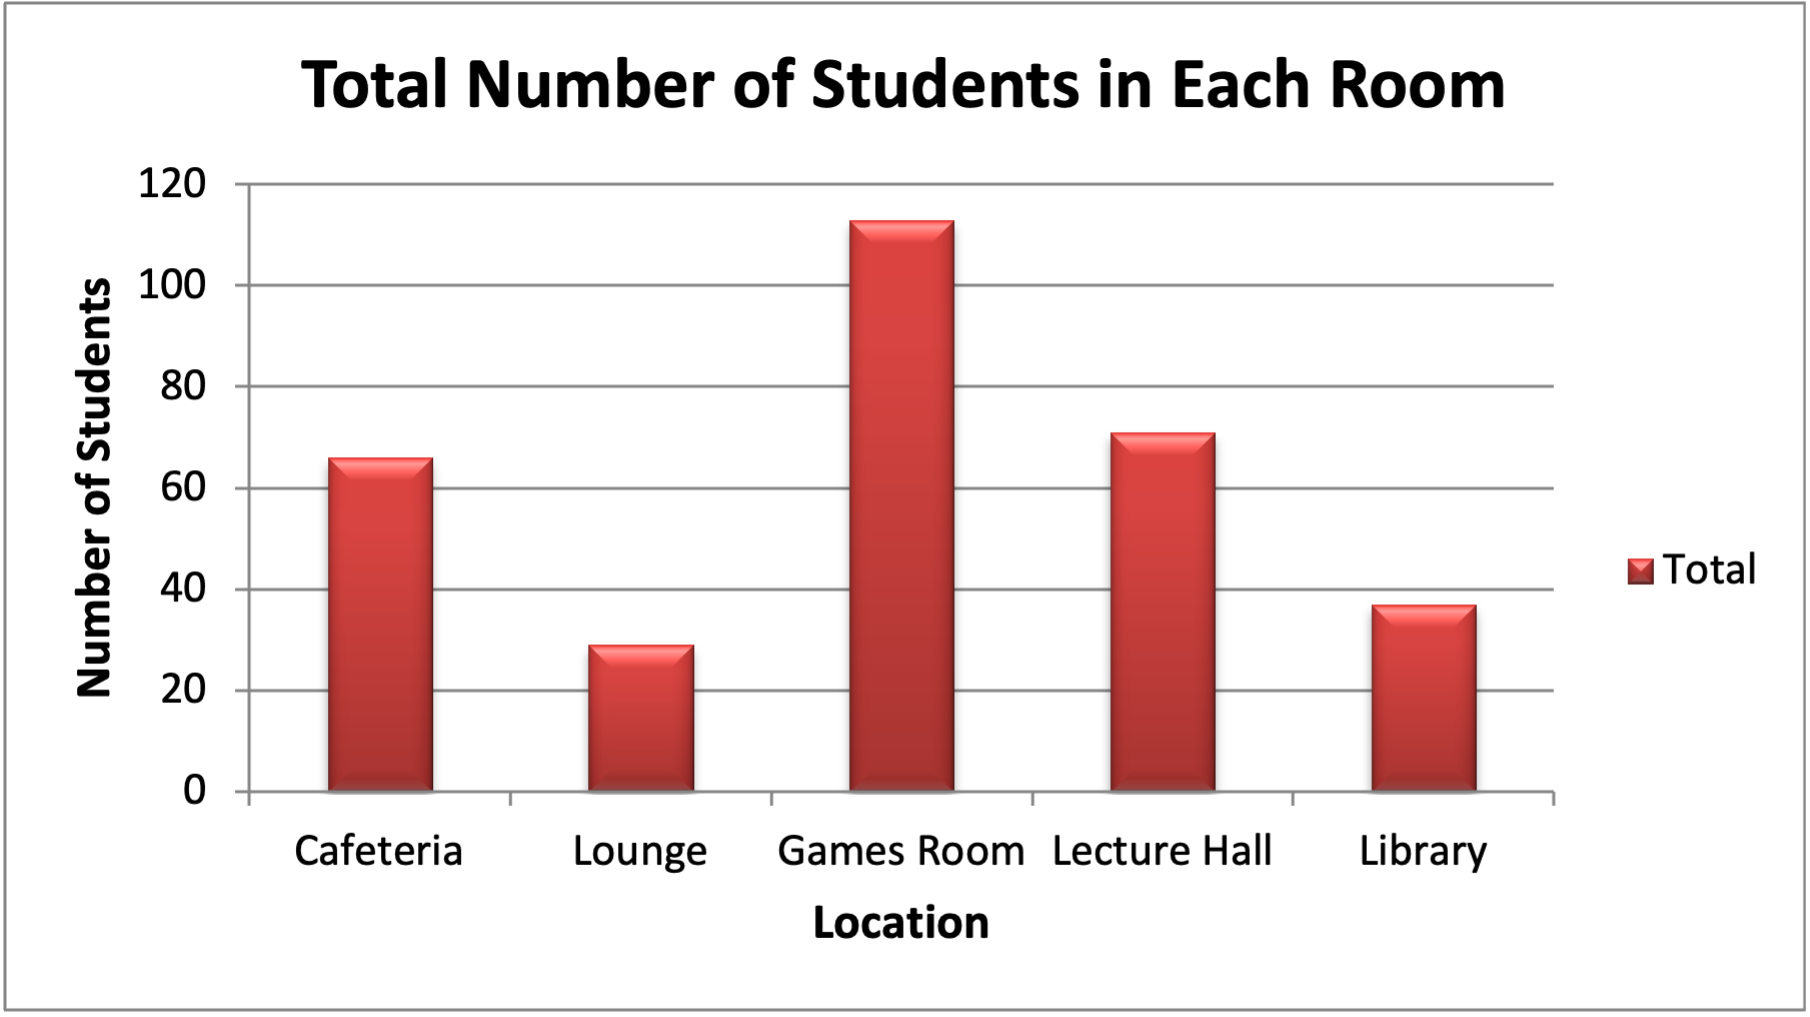
\includegraphics[width=0.9\linewidth]{Exercise1Bar.png}
			\medskip
			\centerline{(a)}
		\end{minipage}\hfill
		\begin{minipage}[t]{0.5\linewidth}\centering
			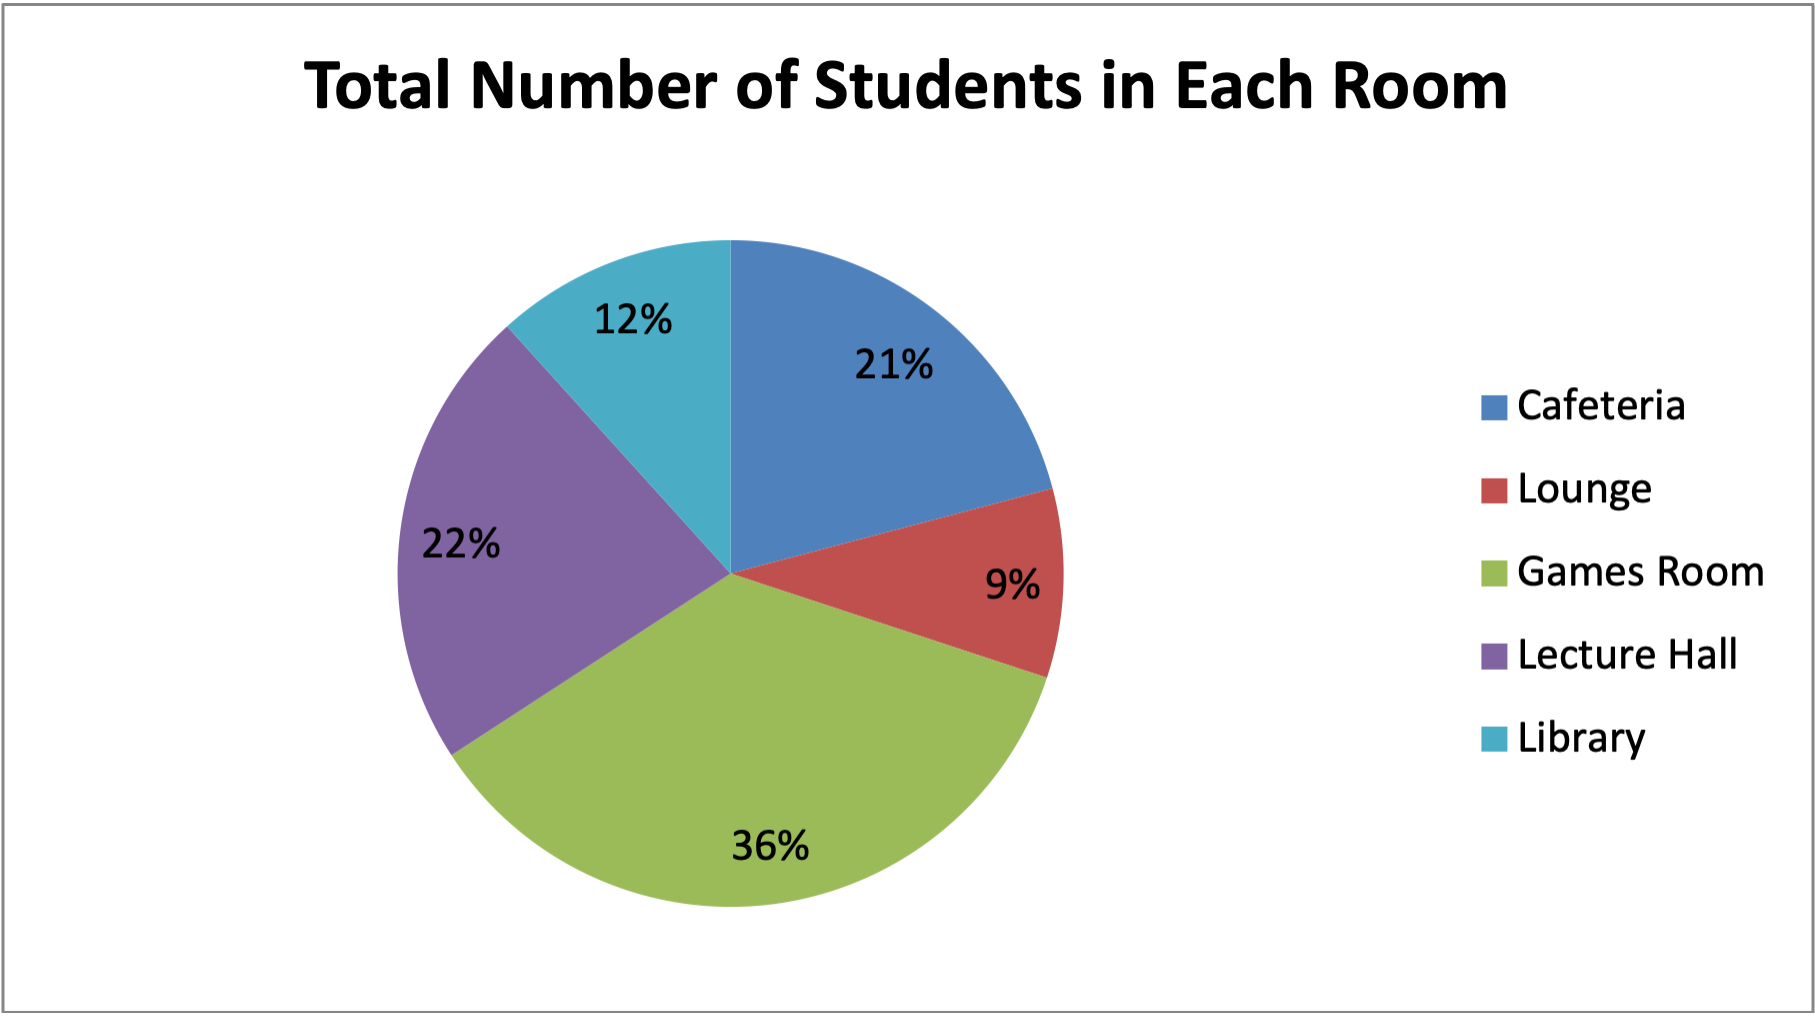
\includegraphics[width=0.9\linewidth]{Exercise1Pie.png}
			\medskip
			\centerline{(b)}
		\end{minipage}
		\begin{minipage}[t]{0.45\linewidth}\centering
			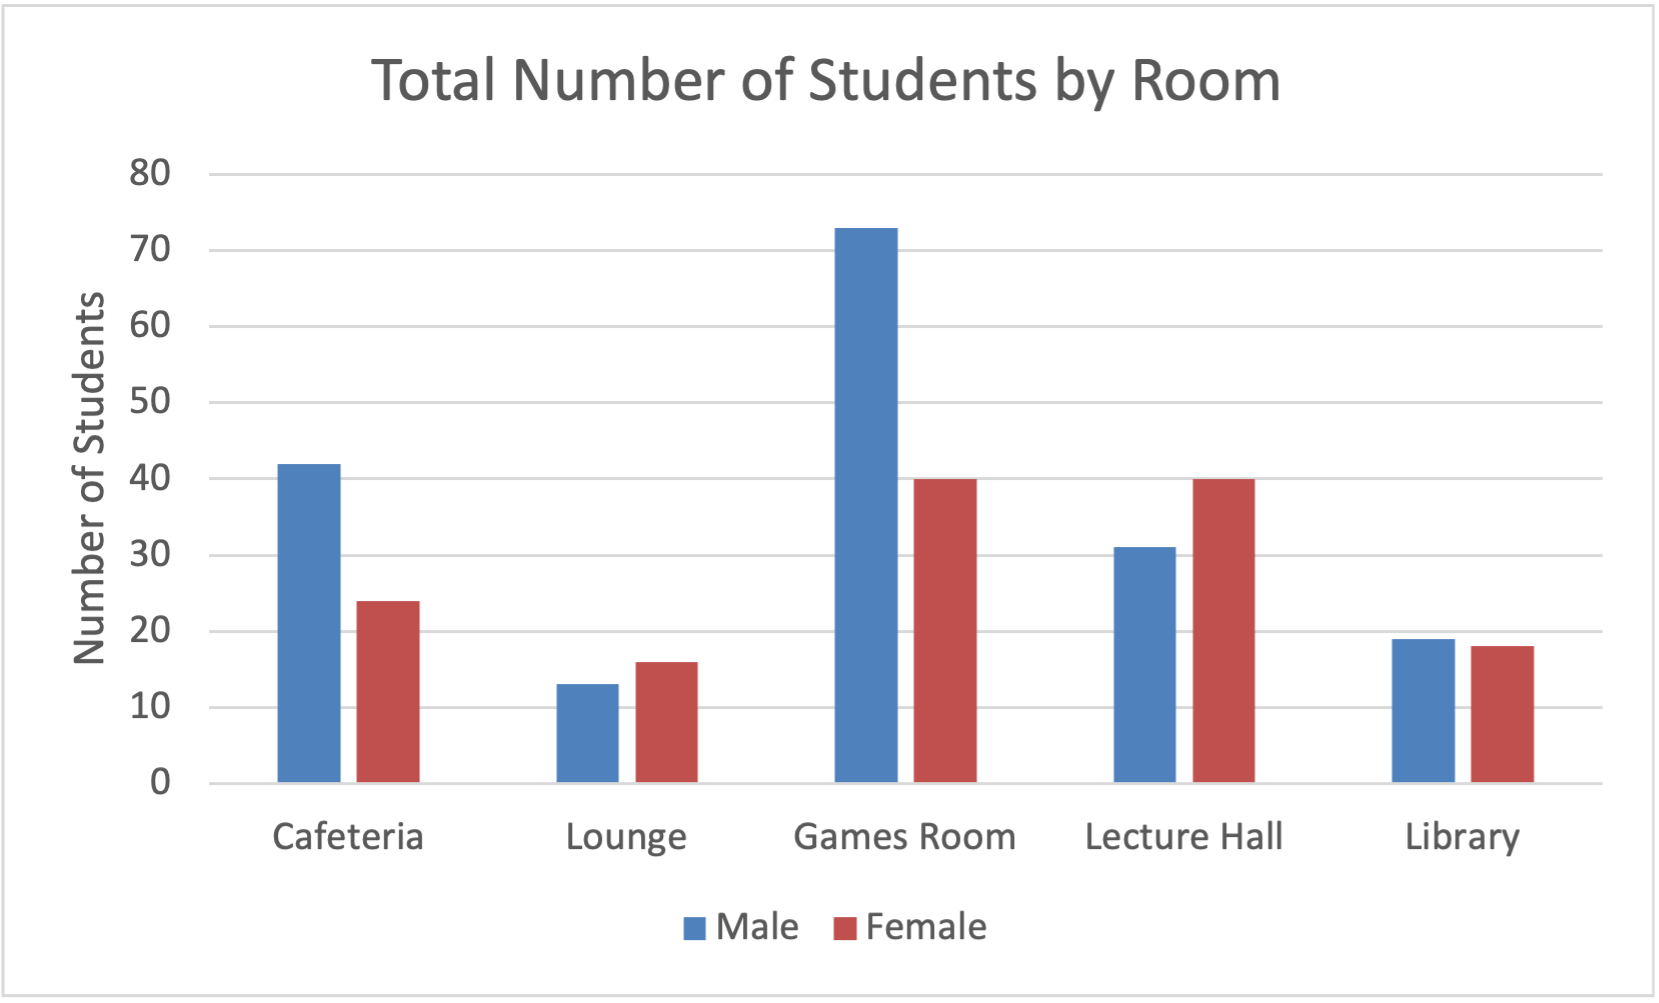
\includegraphics[width=0.9\linewidth]{Exercise1ByRoom.png}
			\medskip
			\centerline{(c)}
		\end{minipage}
		\begin{minipage}[t]{0.45\linewidth}\centering
		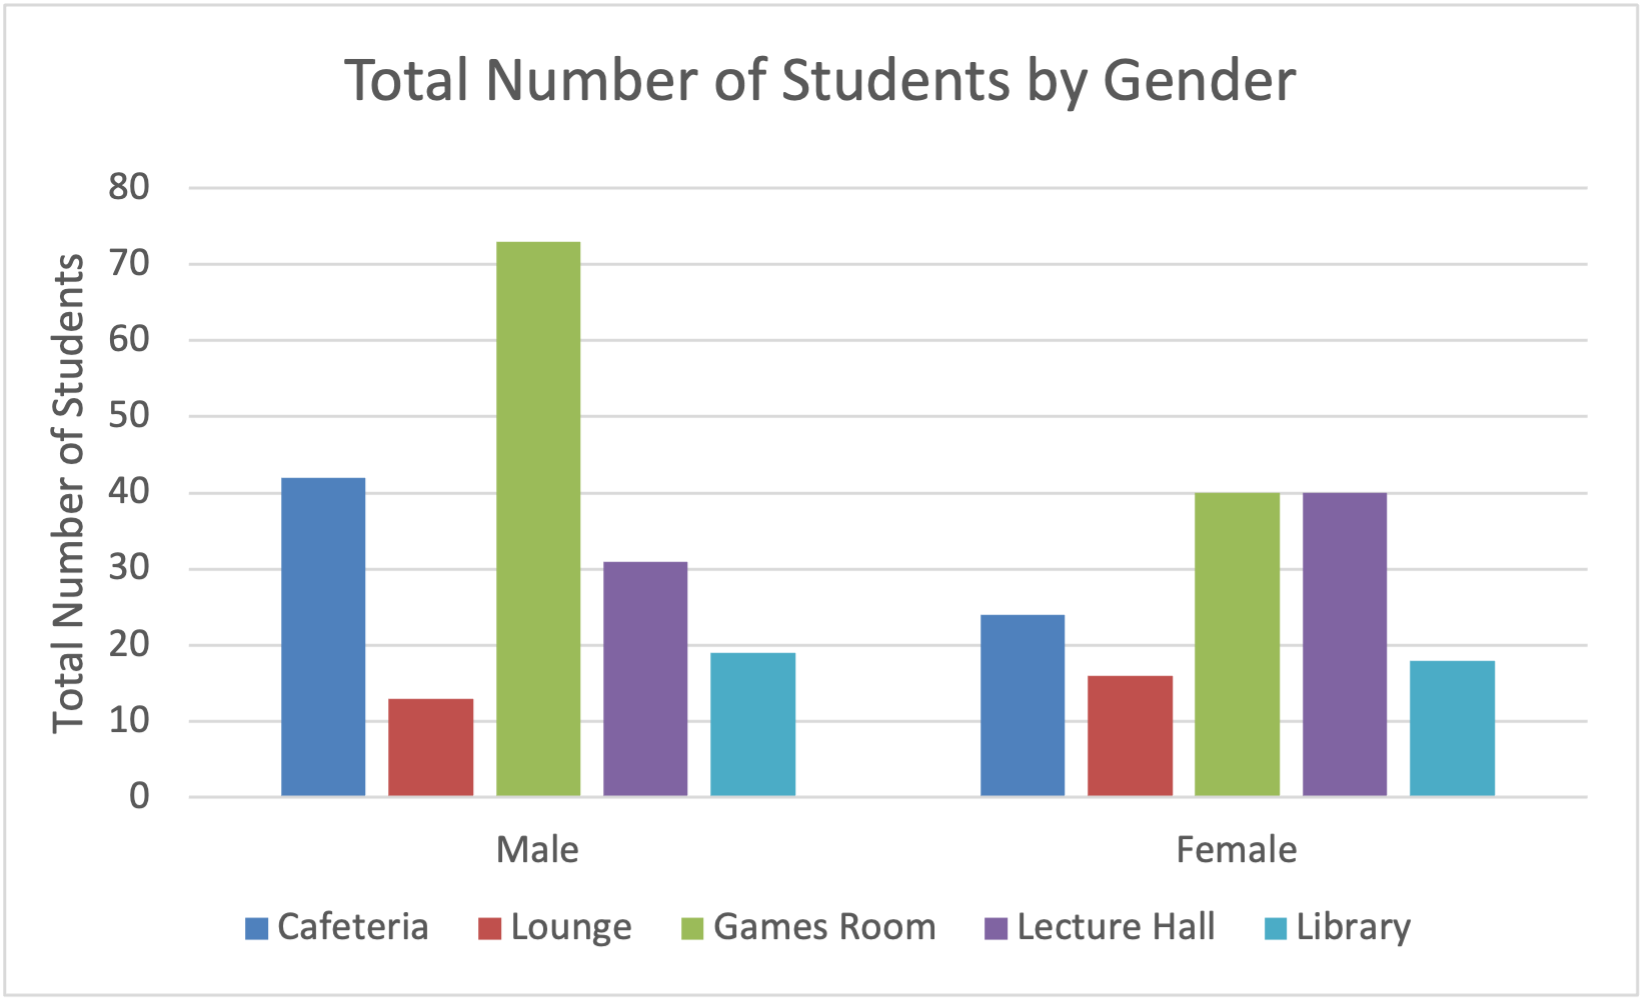
\includegraphics[width=0.9\linewidth]{Exercise1ByGender.png}
		\medskip
		\centerline{(d)}
	\end{minipage}
	\end{figure}
\end{frame}
\section{3-D Charts}
	\begin{frame}
		\frametitle{Formatting 3-D Charts}
		3D charts can be created to show two groupings simulateneously or a 3-D dataset. 
		Try creating a 3-D  Bar Chart by:
		\begin{enumerate}
			\item selecting cells A1:D7 in \textit{ColumnChartExercise.xlsx}
			\item selecting the insert tab, then from selecting the bar chart selecting ``3-D Column Chart"
		\end{enumerate}
	Try creating 3D chart versions of charts (c) and (d) in the previous exercise.
	\end{frame}
\begin{frame}
	\frametitle{Exercise 1: Solution Continued}
	\begin{center}
		\includegraphics[width=0.9\textwidth]{Exercise3DSoln.png}
	\end{center}
\end{frame}

\section{Pie Charts}
\begin{frame}
	\frametitle{Exploding Slices in a Pie}
	Exploding slices in a pie can be used to draw specific attention to certain slices. We can explode an already formed pie chart by 
	\begin{enumerate}
		\item right(Ctrl) clicking the pie slices
		\item Select ``Format Data Series" from the drop down menu
		\item Change the \% explosion from the Format Dataseries pane on the right.
	\end{enumerate}
\end{frame}

	\begin{frame}
		\frametitle{Grouping Slices in a Pie}
		Pie charts are useful for comparing proportions and further understanding sub categories in each category. 
		Create an Exploding pie chart by
		\begin{enumerate}
			\item arranging the values for interpreation by the Pie chart wizard.This includes:
				\begin{itemize}
					\item setting a column header 
					\item arranging data that will be part of the first plot and second plot
					\item assigning appropriate row headers considering that subset of you want to explode.
				\end{itemize}
		\item select the arranged values
		\item left-click ``Insert" ribbon, and select pie chart.
		\item select 2-D pie with an exploded second pie chart.
		\item once the chart is generated right(Ctrl) click the pie chart and select ``Format Data Series" from the drop down menu.
		\item move series between charts until it presents the appropriate data. 
	\end{enumerate}
	\end{frame}

\section{Further Reading}
	\begin{frame}
		\frametitle{Further Reading}
		Computer Applications for Life Sciences Chapter 2, p. 15-20
	\end{frame}
\end{document}
